\documentclass{standalone}
\usepackage{standalone}

\begin{document}
\section{Comparison and Analysis}
\begin{figure}[h]
				\centering
				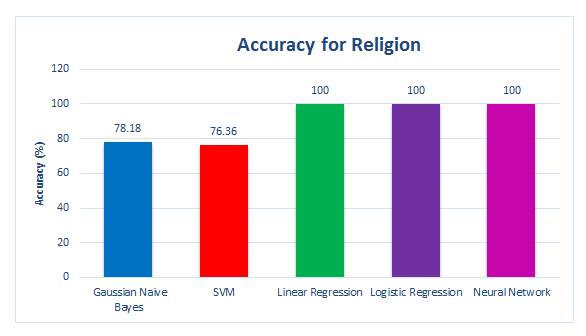
\includegraphics[scale=0.8]{./img/Areligion}
				\caption{Performance diagram of all classification algorithm on Religion.} \label{fig:mapComp}
\end{figure}
From the above diagram we can see that Gaussian Naive Bayes perform well for age, sex, and religion. But it performs very well for sex which is 94.54\% although our data set is small So, choose Gaussian Naive Bayes classifier for sex classification with Facebook snippets. SVM also perform well for Sex and religion. And showed a bad performance for age classification. For religion and sex classification it performs 76.36\% and 87.5\% accuracy respectively. So, we can make decision that sex classification can be classified by Gaussian Naive Bayes model as it performs better than SVM.\\
\begin{figure}[h]
				\centering
				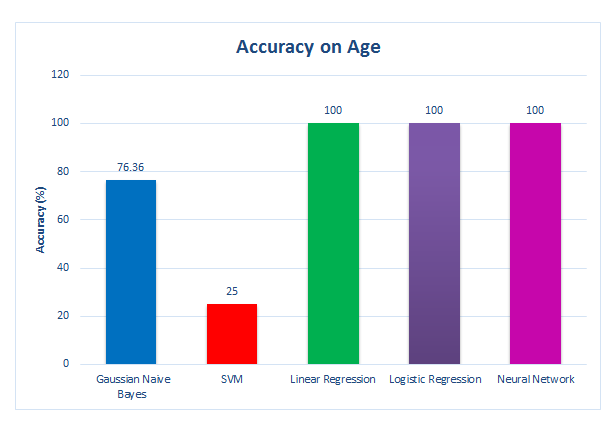
\includegraphics[scale=0.8]{./img/Aage}
				\caption{Performance diagram of all classification algorithm on Age.} \label{fig:mapComp}
\end{figure}
On the other hand, we could not make decision for Artificial Neural Network, Linear Regression and Logistic  Regression although they perform bad in training session. Because size of our data set was not enough big for train those algorithm. 
$
\begin{figure}[h]
				\centering
				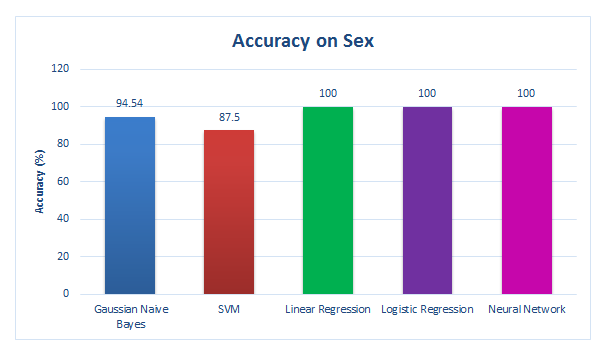
\includegraphics[scale=0.8]{./img/Asex}
				\caption{Performance diagram of all classification algorithm on Sex.} \label{fig:mapComp}
\end{figure}
$
\end{document}